\subsection{Setup Pengujian}
\label{subsection:setup-pengujian}

Sistem yang digunakan dalam pengujian dan juga \textit{benchmark} memiliki konfigurasi yang ditentukan pada file konfigurasi ./etc/config.json. Konfigurasi ini sebelumnya sudah dijelaskan sebagian pada bagian \ref{subsubsection:implementasi-benchmark}.

Untuk masing-masing node, konfigurasi yang ada adalah \textit{ip}, \textit{port}, \textit{port http}, \textit{path} untuk \textit{transaction log}, dan \textit{path} untuk data persisten \textit{key-value store database}. Konfigurasi global yang ada selain konfigurasi masing-masing node adalah \textit{storage}, yaitu jumlah \textit{data shard} dan \textit{parity shard} untuk erasure coding serta ukuran \textit{payload} maksimal yang akan diterima sistem. File konfigurasi yang digunakan dapat dilihat pada gambar \ref{fig:config-json}.

\begin{figure}[ht]
    \centering
    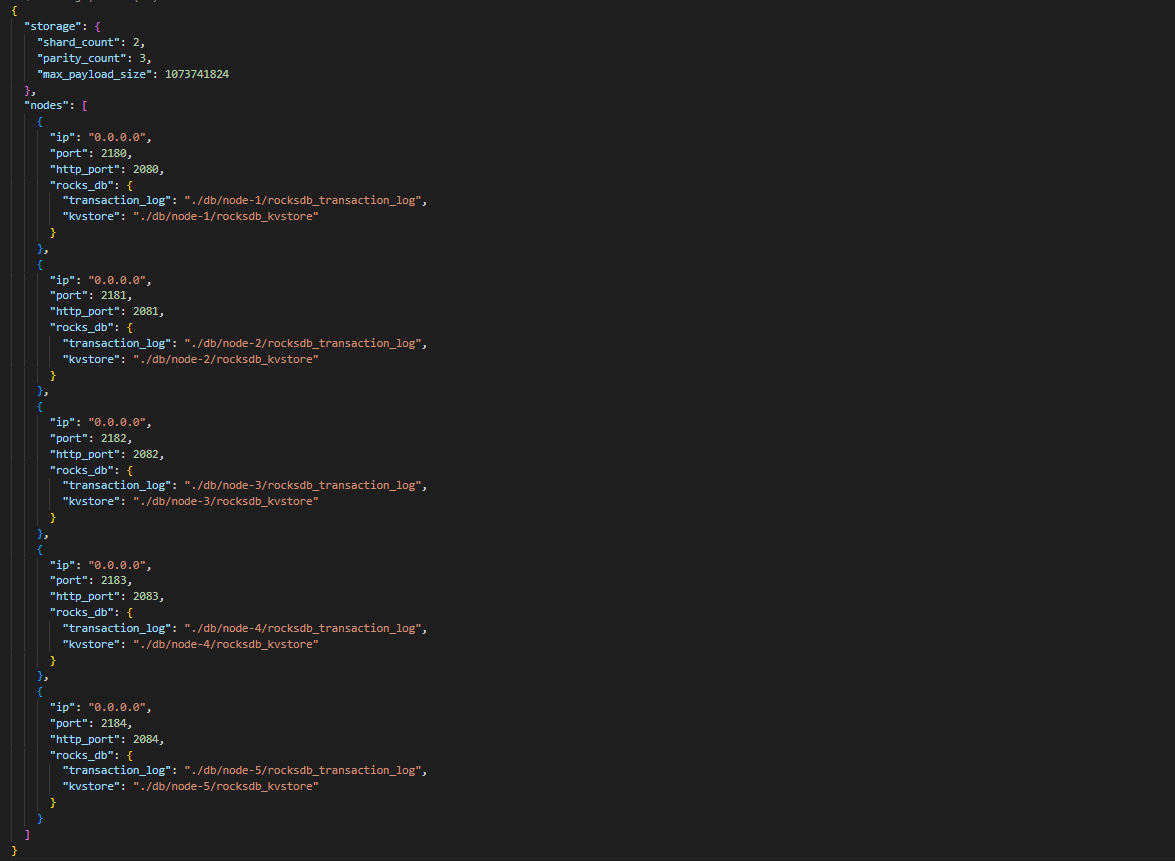
\includegraphics[width=0.95\textwidth]{resources/chapter-4/konfigurasi.png}
    \caption{File konfigurasi yang digunakan}
    \label{fig:config-json}
\end{figure}

Pengaturan sistem untuk menggunakan \textit{erasure coding} atau replikasi tidak ditentukan pada file konfigurasi, tetapi dilakukan saat menjalankan sistem. Pengguna dapat memilih untuk menggunakan \textit{erasure coding} atau
replikasi dengan menggunakan \textit{flag} --erasure untuk \textit{erasure coding} dan tidak menggunakan \textit{flag} tersebut untuk replikasi. Dengan demikian, konfigurasi yang digunakan untuk \textit{erasure coding} dan replikasi adalah sama. Untuk replikasi, jumlah \textit{data shard} dan \textit{parity shard} akan diabaikan dan jumlah keduanya akan dianggap sebagai jumlah \textit{node} secara keseluruhan.